%
% File: chap02.tex
%
\let\textcircled=\pgftextcircled
\chapter{Results}
\label{chap:result}

\initial{I}n this section, the Xenon transient at the GSTR is measured and presented, according to the theory presented in the previous section. Given the procedure limitation, notably the time limitation, the value of the Xenon peak, happening around 7 hours after shutdown, will be guessed.

\section{Results}

The detailed data is presented in appendix~\ref{app:app01}. The xenon reactivity as a function of time is drawn on figure~\ref{fig:xenon}, along with an estimate of the Xenon peak, based on the fact that this peak would have occured roughly 7 hours after shutdown. The graph shows clearly the impact of higher flux on the Xenon distribution in the core, with a sharp decrease of the negative reactivity inserted by the Xenon when the core is at full power.

Is is also interesting to note the positive reactivity inserted by the Xenon at startup. This is due to the high flux at nominal power which eats up the Xenon. In the meantime, $^{135}I$ concentration builds up from nuclear fission of uranium. Eventually, $^{135}Xe$ production from Iodine overtakes its destruction in high flux, hence the increase in negative reactivity after one and a half hour. The Xenon concentration (and consequently the negative reactivity inserted) will eventually reach an equilibrium after 40 to 50 hours.

\begin{figure}[t!]
	\centering
	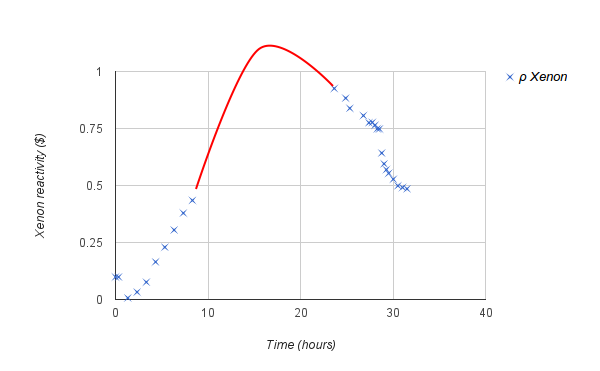
\includegraphics[height=0.4\textheight]{fig02/xenon.png}
	\mycaption[Reactivity of $^{135}Xe$ in the GSTR]{Reactivity of $^{135}Xe$ in the GSTR.}
	\label{fig:xenon}
\end{figure}

\section{Uncertainties}

Several uncertainties sources can be observed in the system. First, the control rod calibration curves and the Xenon-free excess reactivity are given within a certain uncertainty interval, as seen in the previous lab report relative to the transient rod calibration. Moreover, the positions of the rods given in the control room are error-prone, $\pm 2$ steps. All this considered would give an uncertainty of approximately $\pm 0.01\ \$$, or $\pm 1\ cents$, that is roughly $\pm 1\ \%$.

It can be noted that the water temperature impacts the water density and consequently changes the neutron moderation and allows for an improved use of the thermal neutron population. However, this does not impact in any meaningful way the reactivity in the GSTR core. Indeed, the evolution of the temperature that can be observed is not very important in a TRIGA reactor ($\Delta T = 20K$), and it does not translate to any change in the linearity of the antireactivity brought in by the Xenon. This impact is secondary compared to the flux-induced change in Xenon concentration.

Finally, the power is kept stable within a certain margin. An uncertainty on the power translates to an error on the rod positions, hence an error on the reactivity needed to be critical associated. This source of uncertainty can however be considered included in the $\pm 1 \%$ aforementionned.

All in all, the uncertainties relative to this system are relatively limited, and the evolution of the Xenon concentration in the core can be taken with quite high confidence. This is notably due to the long time frame inherent to this experiment, allowing for a certain masking of the uncertainties over time.
